\section{Project Description}
% The ''Portfolio Management Game'' was initially developed in 2001 by an external company for the Department of Banking and Finance at the University of Zurich. This simulation of a portfolio manager was being used from the DBF over several years by multiple seminars of their departement. A course named ''Advanced Portfolio Seminar'' has given insights to the portfolio management process for Master students by playing the game in between different rounds playing the game. For the final seminar of the ''Executive Education'' the game was being played for two days on Uetliberg with all the executive students.\\

%The game has been deprecated by its implemented technologies and after each round the supervisors had to collect a USB-stick where all decisions of the students have been saved to. The supervisors had to collect this data for each group on a central device with administrative access (on a windows native application) to calculate the result of the teams decisions.

%\begin{center}
%  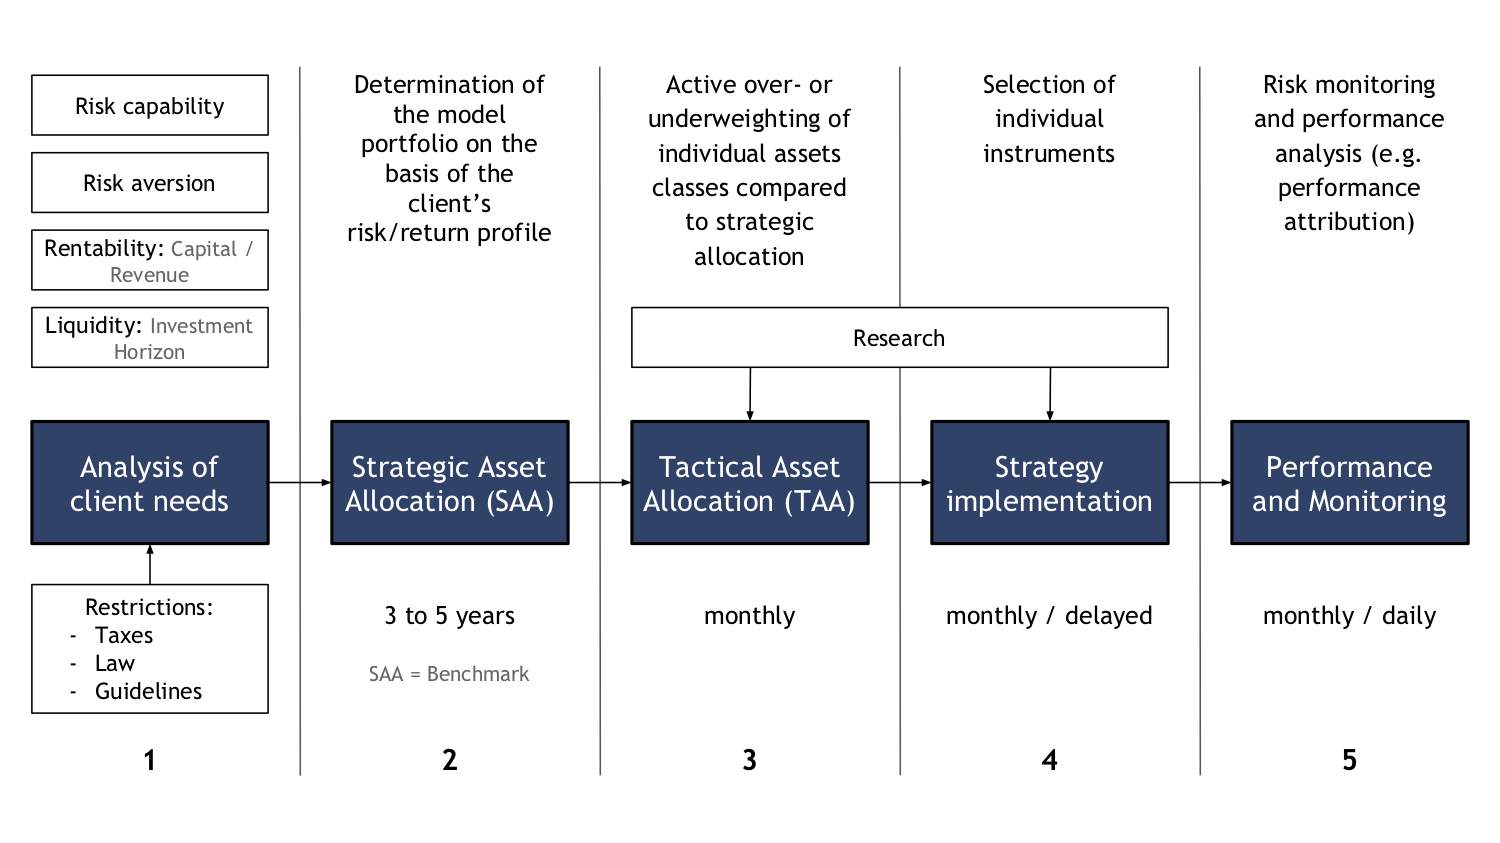
\includegraphics[scale=0.5]{img/private_banking_process.png}
%\end{center}

\subsection{Improvements intentions of the old simulation}
As mentioned in the previous chapter, the current Portfolio Management needs to be revised. According to the involved members of the Department of Banking and Finance, the development of a new simulation intends to enhance different elements and also introduces new features:
\begin{itemize}
  \item For the old solution, specially configured hardware is necessary to play the simulation. The game is based on outdated technologies and after each round, the supervisors had to collect a memory stick where all decisions of the students have been saved onto. The supervisors had to collect this data for each group on a central device with administrative access (on a windows native application) in order to calculate the result of the teams decisions. Especially due to this reason, only a limited amount of teams can play the game simultaneously. Through the transformation into a web-based environment, the simulation can be used independent of time and location, whereby the number of participants can be scaled. It is therefore also conceivable that the simulation can be offered not only to students at the Department of Business, Economics, and Informatics, but also to students of other faculties with appropriate support.
  \item Due to the use of historical, real financial market data in the previous simulation, students can improve their success in the simulation by researching past share prices. This means that currently, not those students who invest the money in a scientifically meaningful way who score best, but those who carry out the best research. A new simulation shall enable the use of data, which is simulated by mathematical processes before the execution. On the one hand, this improves fairness in the simulation and on the other hand, it also shows that it is not possible to forecast financial market data precisely. The simulation of the data lies within the task field of the Department of Banking and Finance Team.
  \item Students should be shown that the forecasting ability of financial markets is limited and that the investment of funds should, therefore, be based on fewer, theoretically sound principles. With the simulation the students that misconduct can lead to short-term profits, but that systematic behaviour is decisive for success in the long term.
\end{itemize}

The first point of the enumeration above is to be addressed from the IT project team (athors of this work) whereas the subsequent two items of the list are the task of the DBF project team.


\subsection{Project Procedure}

The project is first planned by the project management and the specifications for the implementation are defined in cooperation with the IT team. In a second step, a student from the DBF receives the task to prepare the economic model for the data simulation.\\

Thereafter, the IT framework is selected based on the specifications, expert as well as user surveys. In this important phase from an IT view, the simulation is being rebuilt and reprogrammed.\\

A testing and finalization phase follows after the end of this master project. Thereby, the game will be tested by the project team and additionally needed functionalities incorporated.\\

Finally, the finished product will be used for regular study purposes. This simulation of a portfolio manager was being used from the DBF in a course named ''Advanced Portfolio Management Game''. For the final seminar of the Finance Executive Education the game was being played for two days on Uetliberg. As soon as the new simulation is ready, it should be possible to play the portfolio game also within larger classes (e.g. assessment level students).


\subsection{IT Target}
% TODO alternatively include link to user stories?
The main targets for the IT-team are the following aspects:
\begin{itemize}
  \item \textbf{Usability:} The different game sequences within the market model should be well-designed and comprehensible for the game master and the players.
  \item \textbf{Scalability:} Design a well functioning game that can be played with smaller and larger number of students (assessment: in about 700 students in the course Banking \& Finance II).
  \item \textbf{Modularity:} Basic and advanced version(s) allows the game to be used on different levels of study.
\end{itemize}

Important characteristics and components of the game:
\begin{itemize}
  \item The game should be self-explanatory and intuitive.
  \item A brief and concise game documentation is to be created (part of the project report).
  \item The game contains at least the useful components of the old game (except using industry-level instead of single firms).
  \item Informative innovative graphical output (as self-explanatory as possible) for the instructor (based on the current Excel-evaluation and further ideas we provide in advance and students (see ''Teilnehmerbericht'' of the old game and further a depiction of performance-attribution).
  \item New market model created by the Department of Banking and Finance in an Excel spreadsheet which will be the base for the implementation of the authors.
\end{itemize}
